

\tikzset{every picture/.style={line width=0.75pt}} %set default line width to 0.75pt        

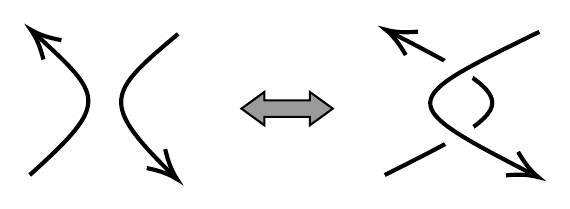
\begin{tikzpicture}[x=0.75pt,y=0.75pt,yscale=-1,xscale=1]
%uncomment if require: \path (0,109); %set diagram left start at 0, and has height of 109

%Curve Lines [id:da9625826323139346] 
\draw [color={rgb, 255:red, 0; green, 0; blue, 0 }  ,draw opacity=1 ][line width=1.5]    (27,88) .. controls (66.2,52.72) and (62.18,50.09) .. (29.53,19.88) ;
\draw [shift={(27.5,18)}, rotate = 402.85] [color={rgb, 255:red, 0; green, 0; blue, 0 }  ,draw opacity=1 ][line width=1.5]    (14.21,-6.37) .. controls (9.04,-2.99) and (4.3,-0.87) .. (0,0) .. controls (4.3,0.87) and (9.04,2.99) .. (14.21,6.37)   ;
%Curve Lines [id:da8544856752658218] 
\draw [color={rgb, 255:red, 0; green, 0; blue, 0 }  ,draw opacity=1 ][line width=1.5]    (95.77,87.82) .. controls (60.17,52.83) and (64.69,48.42) .. (98.5,20) ;
\draw [shift={(98,90)}, rotate = 224.24] [color={rgb, 255:red, 0; green, 0; blue, 0 }  ,draw opacity=1 ][line width=1.5]    (14.21,-6.37) .. controls (9.04,-2.99) and (4.3,-0.87) .. (0,0) .. controls (4.3,0.87) and (9.04,2.99) .. (14.21,6.37)   ;
%Left Right Arrow [id:dp02644365779692881] 
\draw  [fill={rgb, 255:red, 155; green, 155; blue, 155 }  ,fill opacity=1 ] (129,56) -- (140,48) -- (140,52) -- (162,52) -- (162,48) -- (173,56) -- (162,64) -- (162,60) -- (140,60) -- (140,64) -- cycle ;
%Curve Lines [id:da8815340708073711] 
\draw [color={rgb, 255:red, 0; green, 0; blue, 0 }  ,draw opacity=1 ][line width=1.5]    (198,88) .. controls (267.3,53.35) and (266.03,53) .. (200.51,19.04) ;
\draw [shift={(198.5,18)}, rotate = 387.40999999999997] [color={rgb, 255:red, 0; green, 0; blue, 0 }  ,draw opacity=1 ][line width=1.5]    (14.21,-6.37) .. controls (9.04,-2.99) and (4.3,-0.87) .. (0,0) .. controls (4.3,0.87) and (9.04,2.99) .. (14.21,6.37)   ;
%Shape: Circle [id:dp7918407891980368] 
\draw  [draw opacity=0][fill={rgb, 255:red, 255; green, 255; blue, 255 }  ,fill opacity=1 ] (225,38) .. controls (225,33.58) and (228.58,30) .. (233,30) .. controls (237.42,30) and (241,33.58) .. (241,38) .. controls (241,42.42) and (237.42,46) .. (233,46) .. controls (228.58,46) and (225,42.42) .. (225,38) -- cycle ;
%Shape: Circle [id:dp48274841693443793] 
\draw  [draw opacity=0][fill={rgb, 255:red, 255; green, 255; blue, 255 }  ,fill opacity=1 ] (226,69) .. controls (226,64.58) and (229.58,61) .. (234,61) .. controls (238.42,61) and (242,64.58) .. (242,69) .. controls (242,73.42) and (238.42,77) .. (234,77) .. controls (229.58,77) and (226,73.42) .. (226,69) -- cycle ;
%Curve Lines [id:da344766333551638] 
\draw [color={rgb, 255:red, 0; green, 0; blue, 0 }  ,draw opacity=1 ][line width=1.5]    (268.9,87.4) .. controls (202.05,52.99) and (204.04,52.49) .. (272.5,19) ;
\draw [shift={(272,89)}, rotate = 207.22] [color={rgb, 255:red, 0; green, 0; blue, 0 }  ,draw opacity=1 ][line width=1.5]    (14.21,-6.37) .. controls (9.04,-2.99) and (4.3,-0.87) .. (0,0) .. controls (4.3,0.87) and (9.04,2.99) .. (14.21,6.37)   ;




\end{tikzpicture}